\documentclass{article}

\usepackage{amsfonts, amsmath, amssymb, bm} %Math fonts and symbols
\usepackage{dcolumn, multirow} % decimal-aligned columns, multi-row cells
\usepackage[colorlinks=true]{hyperref}
\usepackage{graphicx, subfigure, float} % graphics commands
\usepackage[margin=1in]{geometry} % sets page layout
\usepackage{setspace}% allows toggling of double/single-spacing
\usepackage{verbatim}% defines environment for un-evaluated code
\usepackage{natbib}% defines citation commands and environments.
\singlespace % set document spacing to single
\bibpunct[, ]{(}{)}{,}{a}{}{,} % sets the punctuation of the bibliography entires.
\newcolumntype{d}[1]{D{.}{.}{#1}} % defines a decimal-aligned column
\usepackage{tikz}
\usetikzlibrary{intersections}
\usepackage{enumerate}
\usepackage[utf8]{inputenc}
\usepackage[english]{babel}
\usepackage{minted}
\hyphenpenalty=10000



\begin{document}
\section*{For-loops}
As we tried to explain during the class, in Python, you can iterate over a~list using for-loops in two different ways. However, we are not sure whether everything was clear enough. Hopefully, this short manual will let you understand the difference between iterating over elements and iterating over indexes better. Before we move any further we will talk a~bit about lists. For sure, you remember that in Python you simply define them by writing, for example: 
\begin{center}
    \begin{minted}{python}
        example_list = ["a","b","c","d","e","f"]
    \end{minted}
\end{center}
    
\noindent So actually you can think about it as a~one-dimensional array with six cells. In every single cell you have only one element, hence in the case of \mintinline{python}{example_list} it looks like this:
\begin{center}
    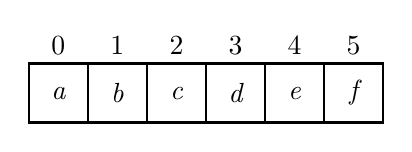
\begin{tikzpicture}[
        list/.style={
            % The shape:
            rectangle,
            % The size:
            minimum size=.75cm,
            % The border
            thick,
            draw=black,
            % The filling
            fill=white,
            % Font
            font=\itshape
        }]

        \foreach \x/\xtext/\xletters in {0/0/a, 0.75/1/b, 1.5/2/c, 2.25/3/d, 3/4/e, 3.75/5/f}
        {
            \node [list]  at (\x,0) {\xletters};
            \node at (\x,.6) {\xtext};
        }
        
    \end{tikzpicture}
\end{center}
\noindent For-loops serve to iterate over every single element in the list and do something to it. Imagine that you would like to print capital letters of all elements in the \mintinline{python}{example_list}. Without a~for-loop you would probably do something like this:

\begin{center}
    \begin{minted}{python}
        print(example_list[0].upper())
        A
        print(example_list[1].upper())
        B
        print(example_list[2].upper())
        C
        print(example_list[3].upper())
        D
        print(example_list[4].upper())
        E
        print(example_list[5].upper())
        F
    \end{minted}
\end{center}

\noindent It would be a really inefficient way of printing the capital letters even for such a shortlist. Therefore, we use for-loops to save time and lines of code.

\subsection*{Iterate over indexes}
The first method does exactly what we did above but we just need to write two lines of code instead of fives:
\begin{center}
    \begin{minted}{python}
        for number in range(len(example_list)):
            print(example_list[number].upper())
        A
        B
        C
        D
        E
        F
    \end{minted}
\end{center}

\noindent Before we start with the for-loop, let's talk a~bit about the \mintinline{python}{range()} \footnote{If you want to learn more about \mintinline{python}{range()} function. Execute the following code in Colab: \mintinline{python}{help(range)}.} function. It takes three arguments but two of them have default values. So in most cases, we feed it with only one argument. But what does it do? It creates a~list-like object of numbers and the argument we usually input is the upper limit of the sequence of these numbers. By default, the lower limit is 0, and the step is 1. It means that when we run for example \mintinline{python}{range(5)}, it creates a~list-like object which contains numbers $0, 1, 2, 3, 4$. However, the important notion is that \mintinline{python}{range()} does not produce a~list and is usually used only in loops.\\

\noindent Knowing what \mintinline{python}{range()} does let's move to the for-loop. In simple words, we created a temporary variable which we called \mintinline{python}{number}. In every step of the loop, Python takes one element from the list-like object produced by \mintinline{python}{range()} and assigns it to the temporary variable \mintinline{python}{number}. So in the first step, it looks like this:

\begin{center}
    \begin{minted}{python}
        number = 0
        print(example_list[number].upper())
        A
    \end{minted}
\end{center}

\noindent In the second iteration like this:

\begin{center}
    \begin{minted}{python}
        number = 1
        print(example_list[number].upper())
        B
    \end{minted}
\end{center}

\noindent And so on and so on, until the for-loop reaches the last element of the list-like object produced by \mintinline{python}{range()}. So actually it does exactly the same thing as you would do. However, it would be highly inefficient and simply a~waste of your time. The important thing you need to remember is that the variable \mintinline{python}{number} lives only inside the for-loop.

\subsection*{Iterate over elements}
The second method takes every single element of the list and does something to it, for example:
\begin{center}
    \begin{minted}{python}
        for letter in example_list:
            print(letter.upper())
        A
        B
        C
        D
        E
        F
    \end{minted}
\end{center}
\noindent But how exactly does it happen? In the first iteration the for-loop assigns the element from the 0~cell to the temporary variable \mintinline{python}{letter}. So in the first step it looks like this:

\begin{center}
    \begin{minted}{python}
        letter = "a"
        print(letter.upper())
        A
    \end{minted}
\end{center}
\noindent In the second iteration like this:
\begin{center}
    \begin{minted}{python}
        letter = "b"
        print(letter.upper())
        B
    \end{minted}
\end{center}
\noindent And so on and so on, until the for-loop reaches the last element. Likewise, in the first method, here the variable \mintinline{python}{letter} lives only in the for-loop.

\end{document}